%TODO: Web Services => web services, php => PHP

\documentclass[10pt,final,a4paper,oneside]{article}
%\documentclass[10pt,journal,final,a4paper,twoside]{IEEEtran}
%\documentclass[10pt,journal,draftclsnofoot,a4paper]{IEEEtran}
%\documentclass[10pt,journal,draftclsnofoot,onecolumn,a4paper]{IEEEtran}
%\documentclass[10pt,journal,final,onecolumn,a4paper]{IEEEtran}

\usepackage{cite}
\usepackage{graphicx}

\begin{document}
\title{Web Services with eZ Components:\\ A Design Proposal}
\author{Falko~Menge and Stefan~Marr}
\markboth{Web Services with eZ Components}{Falko Menge and Stefan Marr}

\maketitle


\begin{abstract}
This Paper describes the current state of design for the InstantSVC core components.
It serves as basis for discussing the contribution of the core components of InstantSVC to eZ components.
\end{abstract}

\section{Web Services and PHP5}\label{sec:Introduction}
Web services are one of the most interesting technologies to evolve in the
last years. They facilitate interoperable communication across the borders of 
platforms and programming languages and are therefore a very 
promising concept for enterprise software. They can be used to integrate 
internal software systems as well as cross-company applications. The main idea is that 
applications provide their functionality in form of services that can be 
used by other applications via network or even internet. 

The standards that form the foundation for Web Services are the SOAP
protocol \cite{SOAP}, the Web Services Description Language (WSDL) \cite{WSDL},
Universal Description, Discovery and Integration (UDDI) \cite{UDDI} and the
Hypertext Transfer Protocol (HTTP) \cite{HTTP}.
SOAP is the messaging protocol used to access the services. WSDL is an
open standard for XML-based service interface descriptions which serve as
contracts between service provider and consumer. Name services for
publishing and searching Web Services are specified by UDDI. HTTP is
leveraged as transport protocol for SOAP messages and in case of RESTful
Web Services it serves as a universal and minimal interface to all
services.

For efficient utilization of SOAP and in most cases also of WSDL
sophisticated tools have been developed for all major programming
languages and platforms. For UDDI mostly commercial products are used.
PHP5 also incorporates a SOAP implementation with support for WSDL
in form of an extension module.

In order to expose a PHP class as Web Service using this SOAP extension
several steps have to be performed.
At first an interface description has to be created using WSDL. This includes
defining XML Schema expressions \cite{XMLSchema} which specify for all data types
used by methods of the class how they should be represented inside SOAP messages.
The methods themselves become WSDL operations which use the XML Schema types.
If documentation should be provided together with the WSDL description,
the developer may copy the source code documentation into the
documentation element of WSDL.
The last step would be to program a PHP application which start a SOAP server
using the WSDL file, passes the class name to this server and tells it to
handle SOAP request arriving via HTTP POST.

Of course, performing this procedure by hand is not what was meant by
convenient tool support.
The SOAP extension is easy to use. However especially writing WSDL manually is not
acceptable for professional developers who want to build service-oriented
architectures with maybe hundreds of services. Other platforms like e.g.
Java EE or .NET typically use annotation mechanisms to tag classes and methods
for publication as web services. The tagged source code is then processed by a
sophisticated tool chain which generates WSDL descriptions, additional source code
for stubs and skeletons and if needed deployment descriptors for the desired
runtime environment.
After that, the services are ready for instant deployment.
Of course PHP needs no stubs because the SOAP client can use the dynamic
features of the language to create response objects at runtime.
However the same dynamic features make it difficult to generate WSDL from PHP
code because there is no type information in it.
The aim of our work was to eliminate the lack of tool support PHP.

The next sections will present each of the components of the tool chain.
The descriptions will focus especially on architecture and design decisions.
Following the development process of eZ components each section is divided in
two parts.
The first part describes the requirements for a component and the other one
specifies a design.



\section{Reflection}\label{sec:Reflection}

The main objective of the Extended Reflection API is to enhance PHP by type information and annotations. Source code documentations often provide information which fulfills very similar purposes. But most times these documentations are informal and only understandable by human beings. phpDocumentor the standard documentation tool for PHP provides a common way to document source code and uses a formal schema which can be processed by a computer.

The Extended Reflection API uses the source code documentation to determine type information and any other information provided via so called doc-tags. Those tags can be used to realize systems which depend on strong type information or additional information to the source code itself. Application scenarios are WSDL generation for Web Services or Aspect-Oriented Programming. Processable additions to the source code in general enable a wide range of new applications. 

\subsection{Requirements}\label{subsec:ReflectionRequirements}
%eZ component: Reflection, Requirements
%~~~~~~~~~~~~~~~~~~~~~~~~~~~~~~~~~
%
%Introduction
%============
Source code documentations often provide information which fulfills very similar purposes. But most times these documentations are not formal and only understandable by human beings. In the PHP world there is a tool called phpDocumentor/PHPDoc which provides a common way to document source code and uses a formal schema which can be processed by a computer.

Application scenarios are WSDL generation for Web Services or Aspect-Oriented Programming. Processable additions to the source code in general enable a wide range of new applications.

Since PHP5 a Reflection API has been included in the standard PHP distribution. It provides an API to get information about classes and all there methods and properties, without the need to parse any source code. Simple functions, runtime objects and PHP Extensions can be inspected, too. But information gathering is not the only feature. It is also possible to modify properties of objects, invoke arbitrary methods/functions and instantiate objects with this Reflection API. With PHP5.1 its capabilities had been enhanced to fulfill all requirements of the Extended Reflection API and it is possible to extract all comments associated to a language construct with API methods at runtime.


Fig. 1. � PHP5 Reflection API

As shown in Fig. 1 the Reflection API conforms to the meta model of an object-oriented programming language. So it is possible to reflect all aspects of a given class or object.

%Description
%-----------
The main objective of the Extended Reflection API is to enhance PHP by type information and annotations.

The Extended Reflection API uses the source code documentation to determine type information and any other information provided via so called doc-tags. 
Those tags can be used to realize systems which depend on strong type information or additional information to the source code itself.

%Current implementation
%----------------------

%Requirements
%============
Therefore, it has the same features, power and performance as the original Reflection API only enhanced by the ability to obtain annotations for classes, functions/methods or properties. This new feature is also used to implement a type system which enables a script to obtain information about the types of parameters, return values and properties.

not enforce any constraints at runtime.

type names as strings

The type system is designed to distinguish between three main types. PrimitiveTypes are all build in types like Integer, Float, String and so on. ArrayTypes are all kinds of arrays and ClassTypes are used to reflect user defined classes. This differentiation has been made in consideration of the language behavior and the capabilities of WSDL for defining types in a language independent way. As arrays are treated in a special way they are additionally classified in simple arrays and maps. Maps are used if the array is an associative array and it is used much like key, value pairs.

%Design goals
%============

%Special considerations
%======================
But this requires a correct source code documentation 
The PHP language runtime is not modified at all. So it is possible that runtime behavior does not correspond with expected behavior caused by improper documentation.

%Format
%======
PHPDoc

%Diagrams
%========

\subsection{Design}\label{subsec:ReflectionDesign}
%eZ component: Reflection, Design
%~~~~~~~~~~~~~~~~~~~~~~~~~~~~~~~~~
%
%Introduction
%============
%
%Description
%-----------

%Design description
%------------------
The Reflection API itself is implemented as a extension written in C for maximum performance and conceptual reasons. The Extended Reflection API is based on this extension and all elements are derived from the given base classes.

Fig. 2. � Extended Reflection API and Type System

In Fig. 2 the Extended Reflection API is shown. For all classes in the Reflection API new subclasses are introduced, which provide new implementations of the inherited methods and additional methods to access type information and annotations.
In addition a new class called ExtendedReflectionAPI is defined, which provides methods necessary to generate Reflection Objects e.g. like getTypeByName. This method will return the appropriate type object for a given type name. For extensibility it is possible to set a different Factory for Type Objects, too. This may be used to extend the provided type system with additional features. Currently it is used for proper type mapping using type names as strings.


API Definitions

\begin{verbatim}
class ExtendedReflectionApi {
    public static ExtendedReflectionApi getInstance()
    public void setTypeFactory(TypeFactory $factory)
    public Type getTypeByName(string $typeName)
}
\end{verbatim}


This global singleton acts as central entry point and factory for reflection by type name. Therefore, it is possible to set a new type factory which could provide enhanced features. If none is provided the standard TypeFactoryImpl is used.

\begin{verbatim}
interface Type {
    function Type getArrayType();
    function Type getMapIndexType();
    function Type getMapValueType();
    function boolean isArray();
    function boolean isClass();
    function boolean isPrimitive();
    function boolean isMap();
    function string toString();
    function boolean isStandardType();
    function string getXmlName();
    function DOMElement getXmlSchema(DOMDocument $dom);
}
\end{verbatim}


The Type interface acts as a central interface for the type system. It is equipped with several methods to reflect attributes about a type. For convenience and usability also methods for an XML Schema mapping are incorporated at this point.

\begin{verbatim}
class ClassType extends ExtReflectionClass implements Type {
    public Type getArrayType()
    public Type getMapIndexType()
    public Type getMapValueType()
    public boolean isArray()
    public boolean isClass()
    public boolean isPrimitive()
    public boolean isMap()
    public string toString()
    public boolean isStandardType()
    public string getXmlName(boolean $usePrefix)
    public DOMElement getXmlSchema(DOMDocument $dom, $namespaceXSD)
    public void __construct(string $name)
}
\end{verbatim}


ClassType is one incarnation of the Type interface. ArrayType and PrimitiveType behave 	similar and are not discussed at this point. Unlike ArrayType and PrimitiveType, the ClassType is tightly integrated with the Extended Reflection API and extends ExtRefelectionClass to inherit all its capabilities.

\begin{verbatim}
class ExtReflectionClass extends ReflectionClass {
    public void __construct(string $name)
    public ExtReflectionMethod getMethod(string $name)
    public ExtReflectionMethod getConstructor()
    public ExtReflectionMethod[] getMethods()
    public ClassType getParentClass()
    public ExtReflectionProperty getProperty(string $name)
    public ExtReflectionProperty[] getProperties()
    public boolean isWebService()
    public string getShortDescription()
    public string getLongDescription()
    public boolean isTagged(string $with)
    public PHPDocTag[] getTags(string $name)
    public ExtReflectionExtension getExtension()
}
\end{verbatim}


ExtReflectionClass inherits from the ReflectionClass and redefines all methods which return a reflection object to return objects from the Extended Reflection API. In addition methods for annotation handling are introduced e.g. getTags, isTagged etc. The general getDocComment method had been superseded by getShortDescription and getLongDescription. This methods return only the part of interest in a PHPDoc comment.


The following classes are analogue to ExtReflectionClass enhancements to the Reflection API and behave very similar.

\begin{verbatim}
class ExtReflectionExtension extends ReflectionExtension {
    public void __construct(string $name)
    public ExtReflectionFunction[] getFunctions()
    public ExtReflectionClass[] getClasses()
}

class ExtReflectionFunction extends ReflectionFunction {
    public void __construct(string $name)
    public ExtReflectionParameter[] getParameters()
    public Type getReturnType()
    public string getReturnDescription()
    public boolean isWebmethod()
    public string getShortDescription()
    public string getLongDescription()
    public boolean isTagged(string $with)
    public PHPDocTag[] getTags(string $name)
}

class ExtReflectionMethod extends ReflectionMethod {
    public void __construct(mixed $class, string $name)
    public ExtReflectionParameter[] getParameters()
    public Type getReturnType()
    public string getReturnDescription()
    public boolean isWebmethod()
    public string getShortDescription()
    public string getLongDescription()
    public boolean isTagged(string $with)
    public PHPDocTag[] getTags(string $name)
    public boolean isMagic()
    public ClassType getDeclaringClass()
}

class ExtReflectionParameter extends ReflectionParameter {
    public void __construct(mixed $mixed, mixed $parameter)
    public Type getType()
    public ClassType getClass()
    public ExtReflectionFunction getDeclaringFunction()
    public ClassType getDeclaringClass()
}

class ExtReflectionProperty extends ReflectionProperty {
    public void __construct(mixed $class, string $name)
    public Type getType()
    public ClassType getDeclaringClass()
}
\end{verbatim}

%Guidelines
%----------

%Algorithms
%----------

%Data structures
%---------------

%Diagrams
%========



\section{CodeAnalyzer}\label{sec:CodeAnalyzer}
%eZ component: CodeAnalyzer, Requirements
%~~~~~~~~~~~~~~~~~~~~~~~~~~~~~~~~~
%
\subsection{Introduction}
%============
The Refletion component provides structural details about
language elements like classes and functions at runtime.
But to be able to use it, those language elements have to be loaded.
Due to the fact that most applications tend to put each class
and function definition in a separate file, it is required to load those files.

\subsubsection{Description}
%-----------
The CodeAnalyzer component is able to load entire class trees
or function libraries into a sandbox environment and to
examine the language elements in them.
In addition to that it is a high level interface to
perform statistical analyses and software metrics with
the Reflection package.

\subsubsection{Current implementation}
%----------------------
The current implementation can be considered as stable
and it meets all requirements which arrised during
development of several tools using it.

\subsection{Requirements}\label{subsec:CodeAnalyzerRequirements}
%============
The component should be able to search through a source tree
and collect information about files respectively classes found.
Some basic software metrics should be implemented.
The required metrics include
counting the lines of code (loc) and the number of
classes, methods, attributes, subclasses and functions.
Furthermore it should collect statistics
about the usage of documentation tags
and warn if important tags are missing.
A possible extension point would be to include abilities
to scan for coding standard violations.

\subsubsection{Design goals}
%============
The component should be easy to use through a convenient high level API
and it should be aware of possible errors in the source code files, i.e.
the CodeAnalyzer should not crash because of syntax errors in a file parsed.
This is very important because if the Code Analyzer would be that instable,
it would only be usefull as a standalone tool for analyzing
smaller applications. It order to become a software metrics library
which can be included in other applications -- such as web service tools --
it has to be reliable.


%Special considerations
%======================

\subsubsection{Format}
%======
The package should at least work with PHP5 source code.

%Diagrams
%========

\subsection{Design}\label{subsec:CodeAnalyzerDesign}
%eZ component: CodeAnalyzer, Design
%~~~~~~~~~~~~~~~~~~~~~~~~~~~~~~~~~
%
%Introduction
%============
%
%Description
%-----------

\subsubsection{Design description}
%------------------
The Code Analyzer should should be based on the reflection component
as a high level API for language elements.
This way it leverages the internal parser of the PHP interpreter
which can be assumed to be one of the best parsers for the language.

The requirement of being fault tolerant has a major influence
on the design of the component.
Since the source files have to be loaded
to employ the reflection component, some kind
of a sandbox environment is needed to ensure the errors
in the input files which stop the script execution
do not affect the Code Analyzer in its execution.

A simple way to achieve this is to start the analysis of the files
in a separate PHP interpreter.
Then in case of errors only this child process stops,
but the Code Analyzer is able to report the error
and to continue with the next file.

The component consists of three classes.

\paragraph{ezcCodeAnalyzer}
ezcCodeAnalyzer is the main class of the component.
It implements the different analyses which can be started either
separately using one of the summarization methods
or all together by calling a central collector method.

\begin{figure}[htbp]
	\centering
		\includegraphics[width=1.00\textwidth]{figures/callgraph-code_analyzer.ps}
	\caption{Static call graph for class ezcCodeAnalyzer}
	\label{fig:callgraph-code_analyzer}
\end{figure}


%Method Summary 
%\begin{verbatim}
%+static void collectMethodsStats ($classes) 
%~static int countClassesSeeingMethods 
%(array<string, mixed> $classes,  &$methodCount, int $methodCount) 
%~static int countClassesSeeingProperties
%(array<string, mixed> $classes,  &$propCount, int $propCount) 
%~static int countInheritedMethods
%(array<string, mixed> $classes) 
%~static int countOverriddenMethods
%(array<string, mixed> $classes) 
%+static int countPossibleOverriddes
%(array<string, mixed> $classes) 
%+static int countSubclasses (array<string, mixed> $classes, 
%string $class) 
%+static array<string, mixed> summarizeClasses (array<string, mixed> $classes) 
%+static array<string, mixed> summarizeClassMethods (iscReflectionClassType $class, 
% &$missingMethodComments,  &$missingParamTypes, 
%integer $missingMethodComments, integer $missingParamTypes) 
%+static array<string, mixed> summarizeClassProperties
%(iscReflectionClassType $class) 
%+static array<string, mixed> summarizeClassSignature
%(iscReflectionClassType $class) 
%+static array<string, mixed> summarizeFile (string $filename) 
%+static array<string, mixed> summarizeFunctionParameters  (iscReflectionFunction $method,  &$paramFlaws, integer $paramFlaws) 
%+static array(string=>mixed) summarizeFunctions (string[] $functions) 
%static array<string, mixed> +summarizeInSandbox ( $filename, string[] $classes) 
%+static array(string=>mixed) summarizeInterfaces (string[] $interfaces) 
%+iscCodeAnalyzer __construct ([string $path = '.']) 
%~void buildInheritanceTree () 
%+void collect () 
%~void collectClassStats () 
%~void collectFunctionStats () 
%~array flatoutStatsArray (array $array, string $basekey) 
%+array getCodeSummary () 
%+array getStats () 
%~void inspectFiles (string[] $files) 
%~void parseDir (string $path,  &$statsArray, array $statsArray) 
%+void summarizeProject ()
%\end{verbatim}

\paragraph{ezcCodeAnalyzerClassLoader}
This class provides methods to recursively include
all files that contain PHP code from a given directory.
Any output of the included code will be suppressed
and files are only loaded if they do not contain
any syntax errors.
This fault tolerance is achieved by creating a new PHP process
and performing a syntax check.

%\verb|public static void loadDir (string $path)| 
%\verb|public static void loadFile (string $file)|


\paragraph{ezcCodeAnalyzerFileDetails}
The class ezcCodeAnalyzer uses this struct as data structure for some details of a file.
The constructor of collects ::: Guessing MimeType, counting lines of code, and retrieving file size are 
done. 

%TODO: maybe leave it out
%\begin{figure}[htbp]
%	\centering
%		\includegraphics[width=1.00\textwidth]{figures/callgraph-file_details-with-external-calls.ps}
%	\caption{Static call graph for class ezcCodeAnalyzerFileDetails}
%	\label{fig:callgraph-file_details-with-external-calls}
%\end{figure}

%\verb|iscCodeAnalyzerFileDetails| extends \verb|ezcBaseStruct|
%
%
%Variable Summary (all protected)
%
%\begin{verbatim}
%int $countClasses <#$countClasses> 
%int $countFunctions <#$countFunctions> 
%int $countInterfaces <#$countInterfaces> 
%string $fileName <#$fileName> 
%int $fileSize <#$fileSize> 
%int $linesOfCode <#$linesOfCode> 
%string $mimeType <#$mimeType>
%\end{verbatim}
%
%
%Method Summary 
%
%\verb|public iscCodeAnalyzerFileDetails __construct ([string $file = ''])|
%
%
%Guess the mime type using the file extension 
% 
%\verb|protected boolean guessMimeType (string $file)|
% 
% 
%Use mime type to decide wheter the lines of code are counable 
% 
%\verb|protected boolean shouldCountLines (string $mime)|


%Guidelines
%----------

\subsubsection{Algorithms}
%----------

The static call graph in figure \ref{fig:callgraph-code_analyzer}
gives an impression of the collaboration between the methods.
In some methods recursion is used for traversing hierarchical 
directory and class structures but most of the algorithms
are not very complex. They simply collect statistics while
leveraging the Reflection component.

\subsubsection{Data structures}
%---------------

%Diagrams
%========



\section{WSDL}\label{sec:WSDL}
\subsection{Introduction}
The Web Services Description Language (WSDL) \cite{WSDL} is one of the most important standards for professional web service applications because it allows for automated creation of SOAP servers and clients. The SOAP extension of PHP5 supports this if a WSDL file is provided. A WSDL file is an XML document describing the interface of a Web Service. A service provider can offer this description to its clients which are then able to determine the operations provided by the service and the messages they have to sent. In this scenario the WSDL document serves as a contract between server and client and both parties have to abide by it in order to communicate successfully.

Although it is possible to write WSDL documents by hand the additional time and effort do not result in a major advantage. Due to the fact that nearly all information needed for a WSDL description already exists in the source code of the class or the functions implementing the Web Service the complete service description can be generated automatically. The only new information in a WSDL file is the binding and the service access point URL.

\subsubsection{Description}
The WSDL component generates a WSDL document from a given service implementation.

\subsubsection{Current implementation}
The WSDL component should be able to generate a WSDL document from a given service implementation. Just like the SOAP server of PHP5 it should accept a class or a set of functions as a service implementation.

\subsection{Requirements}\label{subsec:WSDLRequirements}
%eZ component: WSDL, Requirements
%~~~~~~~~~~~~~~~~~~~~~~~~~~~~~~~~~
%
%Introduction
%============
%
%Description
%-----------
%The WSDL component generates a WSDL document from a given service implementation.
%
%Current implementation
%----------------------
The WSDL component should be able to generate a WSDL document from a given service implementation. Just like the SOAP server of PHP5 it should accept a class or a set of functions as a service implementation.

%Requirements
%============


To be interoperable with other platforms the WSDL component should conform to the Basic Profile of the Web Services-Interoperability Organization (WS-I) \cite{BasicProfile}.

Documentation

%Design goals
%============

Since the generator knows all details about a service it could provide convenience methods for creating a SOAP server.

%Special considerations
%======================
WSDL 1.1

When the WSDL 2.0 specification \cite{WSDL20} is finished the WSDL component could be enhanced to support this as well.

%Format
%======

%Diagrams
%========

\subsection{Design}\label{subsec:WSDLDesign}
%eZ component: WSDL, Design
%~~~~~~~~~~~~~~~~~~~~~~~~~~~~~~~~~
%
%Introduction
%============
%
%Description
%-----------
%The WSDL component generates a WSDL document from a given service implementation.
The WSDL generator leverages the Reflection component. It uses the Document Object Model to create WSDL in a very structured way.


Web Services Interoperability Tests of the SOAP Builders community 


%Design description
%------------------

%Guidelines
%----------

%Algorithms
%----------
\begin{figure}[htbp]
	\centering
		\includegraphics[width=1.00\textwidth]{figures/callgraph-Generators-class.WSDLGenerator.ps}
	\caption{Static call graph of class ezcWSDL}
	\label{fig:callgraph-Generators-class.WSDLGenerator}
\end{figure}


%Data structures
%---------------

%Diagrams
%========



\section{SOAP}\label{sec:SOAP}
\subsection{Requirements}\label{subsec:SOAPRequirements}
%eZ component: SOAP, Requirements
%~~~~~~~~~~~~~~~~~~~~~~~~~~~~~~~~~
%
%Introduction
%============

%Description
%-----------

%Current implementation
%----------------------

%Requirements
%============

%Design goals
%============

%Special considerations
%======================

%Format
%======

%Diagrams
%========

\subsection{Design}\label{subsec:SOAPDesign}
%eZ component: SOAP, Design
%~~~~~~~~~~~~~~~~~~~~~~~~~~~~~~~~~
%
%Introduction
%============
%
%Description
%-----------

%Design description
%------------------

%Guidelines
%----------

\subsubsection{Algorithms}
%----------
\begin{figure}[htbp]
	\centering
		\includegraphics[width=1.00\textwidth]{figures/callgraph-SoapClient-class.SecureClient-with-external-calls.ps}
	\caption{Static call graph for class ezcSecureSoapClient}
	\label{fig:callgraph-SoapClient-class.SecureClient-with-external-calls}
\end{figure}


%Data structures
%---------------

%Diagrams
%========



\section{REST}\label{sec:REST}
\subsection{Requirements}\label{subsec:RESTRequirements}
%eZ component: REST, Requirements
%~~~~~~~~~~~~~~~~~~~~~~~~~~~~~~~~~
%
%Introduction
%============

%Description
%-----------

%Current implementation
%----------------------

%Requirements
%============

%Design goals
%============

%Special considerations
%======================

%Format
%======

%Diagrams
%========

\subsection{Design}\label{subsec:RESTDesign}
%eZ component: REST, Design
%~~~~~~~~~~~~~~~~~~~~~~~~~~~~~~~~~
%
%Introduction
%============
%
%Description
%-----------

%Design description
%------------------

%Guidelines
%----------

%Algorithms
%----------

%Data structures
%---------------

%Diagrams
%========



\section{WebService}\label{sec:WebService}
\subsection{Requirements}\label{subsec:WebServiceRequirements}
%eZ component: WebService, Requirements
%~~~~~~~~~~~~~~~~~~~~~~~~~~~~~~~~~
%
%Introduction
%============

%Description
%-----------

%Current implementation
%----------------------

%Requirements
%============

%Design goals
%============

%Special considerations
%======================

%Format
%======

%Diagrams
%========

\subsection{Design}\label{subsec:WebServiceDesign}
%eZ component: WebService, Design
%~~~~~~~~~~~~~~~~~~~~~~~~~~~~~~~~~
%
%Introduction
%============
%
%Description
%-----------

%Design description
%------------------

%Guidelines
%----------

%Algorithms
%----------

%Data structures
%---------------

%Diagrams
%========



\section{Conclusion}
The extension of PHP's reflection API allowed a very elegant 
implementation of a proffessional WSDL generator. The major advantage of 
this approach is that the algorithms for retrieving type information are 
not tied into the WSDL generator. Instead the new reflection API is a 
reusable building block which already became a foundation for a whole 
family of Web Service helpers. But its fearures are of interest for 
other PHP projects as well. The annotation mechanism could be a basis 
for using new dynamic programming techniques like e.g. aspect-oriented 
programming with PHP. 

The WSDL generator implements the complete WSDL 1.1 standard and 
supports all types of bindings. It conforms to the WS-I Basic Profile 
which guarantees interoperability with Web Service tools of other 
platforms. 

In order to select classes and methods for publication as Web Services 
annotations can be used similar to Java EE or .NET. Semantical details 
taken from the source code documentation can be introduced to generated 

For document/wrapped Web Services adapter classes which handle the 
wrapping and unwrapping can be generated. 

Besides WSDL there are over 20 other Web Service standards concerning 
different anspects like e.g. security, synchronization and sessioning. 
Those standards have in common that they add elements to the SOAP 
header. Therefore, the SOAP component introduces a handler chain 
mechanism allowing for injection of SOAP intermediaries to the 
communication channel. This way WS-* standards can be used with PHP. A 
first standard implemented on top of this platform is WS-Security with 
the Username Token Profile as a first profile providing secure 
authentication for Web Services. 

As an alternative to Web Services with complex SOAP stacks and the 
resulting time and effort RESTful Web Services are gaining popularity 
especially among developers. On the one hand, they are easy to learn and 
do not require large tool chains. On the other hand, the architectural 
concept provides enhanced interoperability. As a reaction to those 
technological developents a REST server has been designed which is able 
to host multiple services and to perform authentication using HTTP 
Digest. 

The Web Service component all proposed components into one convenience 
library which allows automatic generation of SOAP and REST servers from 
existing PHP applications. On top of that professional SOA developers 
can dynamically adapt their service landscapes to the constantly 
changing requirements. 

The InstantSVC project will continue to maintain a web frontend for the 
Web Service component and some commandline tools for the Code Analyzer. 


Since eZ Components is designed for enterprise PHP application development
it should definitely/undoubtedly incorporate professional Web Service components.



\begin{thebibliography}{1}

\bibitem{SOAP}
\emph{SOAP Version 1.2 specification}, W3C Recommendation \hskip 1em plus
  0.5em minus 0.4em\relax World Wide Web Consortium (W3C), June 24, 2003.
  \newline http://www.w3.org/TR/soap/
  
\bibitem{WSDL}
\emph{Web Services Description Language (WSDL) 1.1}, W3C Note \hskip 1em plus
  0.5em minus 0.4em\relax World Wide Web Consortium (W3C), March 15, 2001.
  \newline http://www.w3.org/TR/wsdl

\bibitem{WSDL20}
\emph{Web Services Description Language (WSDL) 2.0}, W3C Candidate Recommendation \hskip 1em plus
  0.5em minus 0.4em\relax World Wide Web Consortium (W3C), March 26, 2006.
  \newline http://www.w3.org/TR/wsdl20

\bibitem{UDDI}
  
\bibitem{BasicProfile}
\emph{Basic Profile Version 1.2} \hskip 1em plus
  0.5em minus 0.4em\relax Web Services-Interoperability Organization (WS-I), Oktober 03, 2006.
  \newline http://www.ws-i.org/Profiles/BasicProfile-1.2.html
  
\bibitem{XMLSchema}

\bibitem{HTTP}

\end{thebibliography}

\end{document}